\chapter{Experimental Setup}\label{chap:exp_setup}
Every theory needs to have experimental proof to show it's compatibility. Particle physics is tested at
the colliders.

This chapter is devided into three parts.
The first part is devoted to the description of the Large Hadron Collider. The second part of the 
chapter is revealing the CMS detector construction and features in more detail how it was used to produce the final
results of this work. The third and the last part of this chapter is about the upgrade plans for the
CMS detector to operate with higher energies and luminosities.

%%%%%%%%%%%%%%%%%%%%%%%%%%%%%%%%%%%%%%
%%%%%%%%%%%%%%%%%%%%%%%%%%%%%%%%%%%%%%
%%%%%%%%%%%%%%%%%%%%%%%%%%%%%%%%%%%%%%
\section{Large Hadron Collider}\label{sec:LHC}

The fastest protons in the world, ever controlled by mankind, are alive in Switzerland at CERN.
The Machine which can manage the operation of these protons is called Large Hadron Collider(LHC). 
The LHC is a ring-shape tunnel 26.7 km long  placed 45 - 170 m underground. 
Inside the tunnel there are two rings with vacuum tubes where proton(or lead nuclei) beams are circulating in different directions.
There are four locations where the rings are crossing and the protons can collide with each other. 
The designed center-of-mass energy for those collisions is $\sqrt{s}$ = 14 TeV, which means 7 TeV per colliding proton.

The protons are guided around the ring by 8 T superconducting magnets. 
For optimal usage of the LHC one needs to preaccelerate and preform the proton bunches.
For this purpose LHC is supported by preacceleration system.


The way of the protons literally starts from a bottle of hydrogen gas.
H$_{2}$ molecules are entering a duoplasmatron proton source\cite{Scrivens:1382102} where they are stripped off the electrons. 
The protons produced by the source have to go through the chain of preaccelerators to satisfy very stringent needs of the LHC -- 
many high intensity proton bunches (2808 per LHC ring) with small transverse and well defined longitudinal emittances.
The following acceleration injector chain is used for the LHC (fig. \ref{fig:AccelCERN}): 

\begin{figure}[t]
  \centering
  %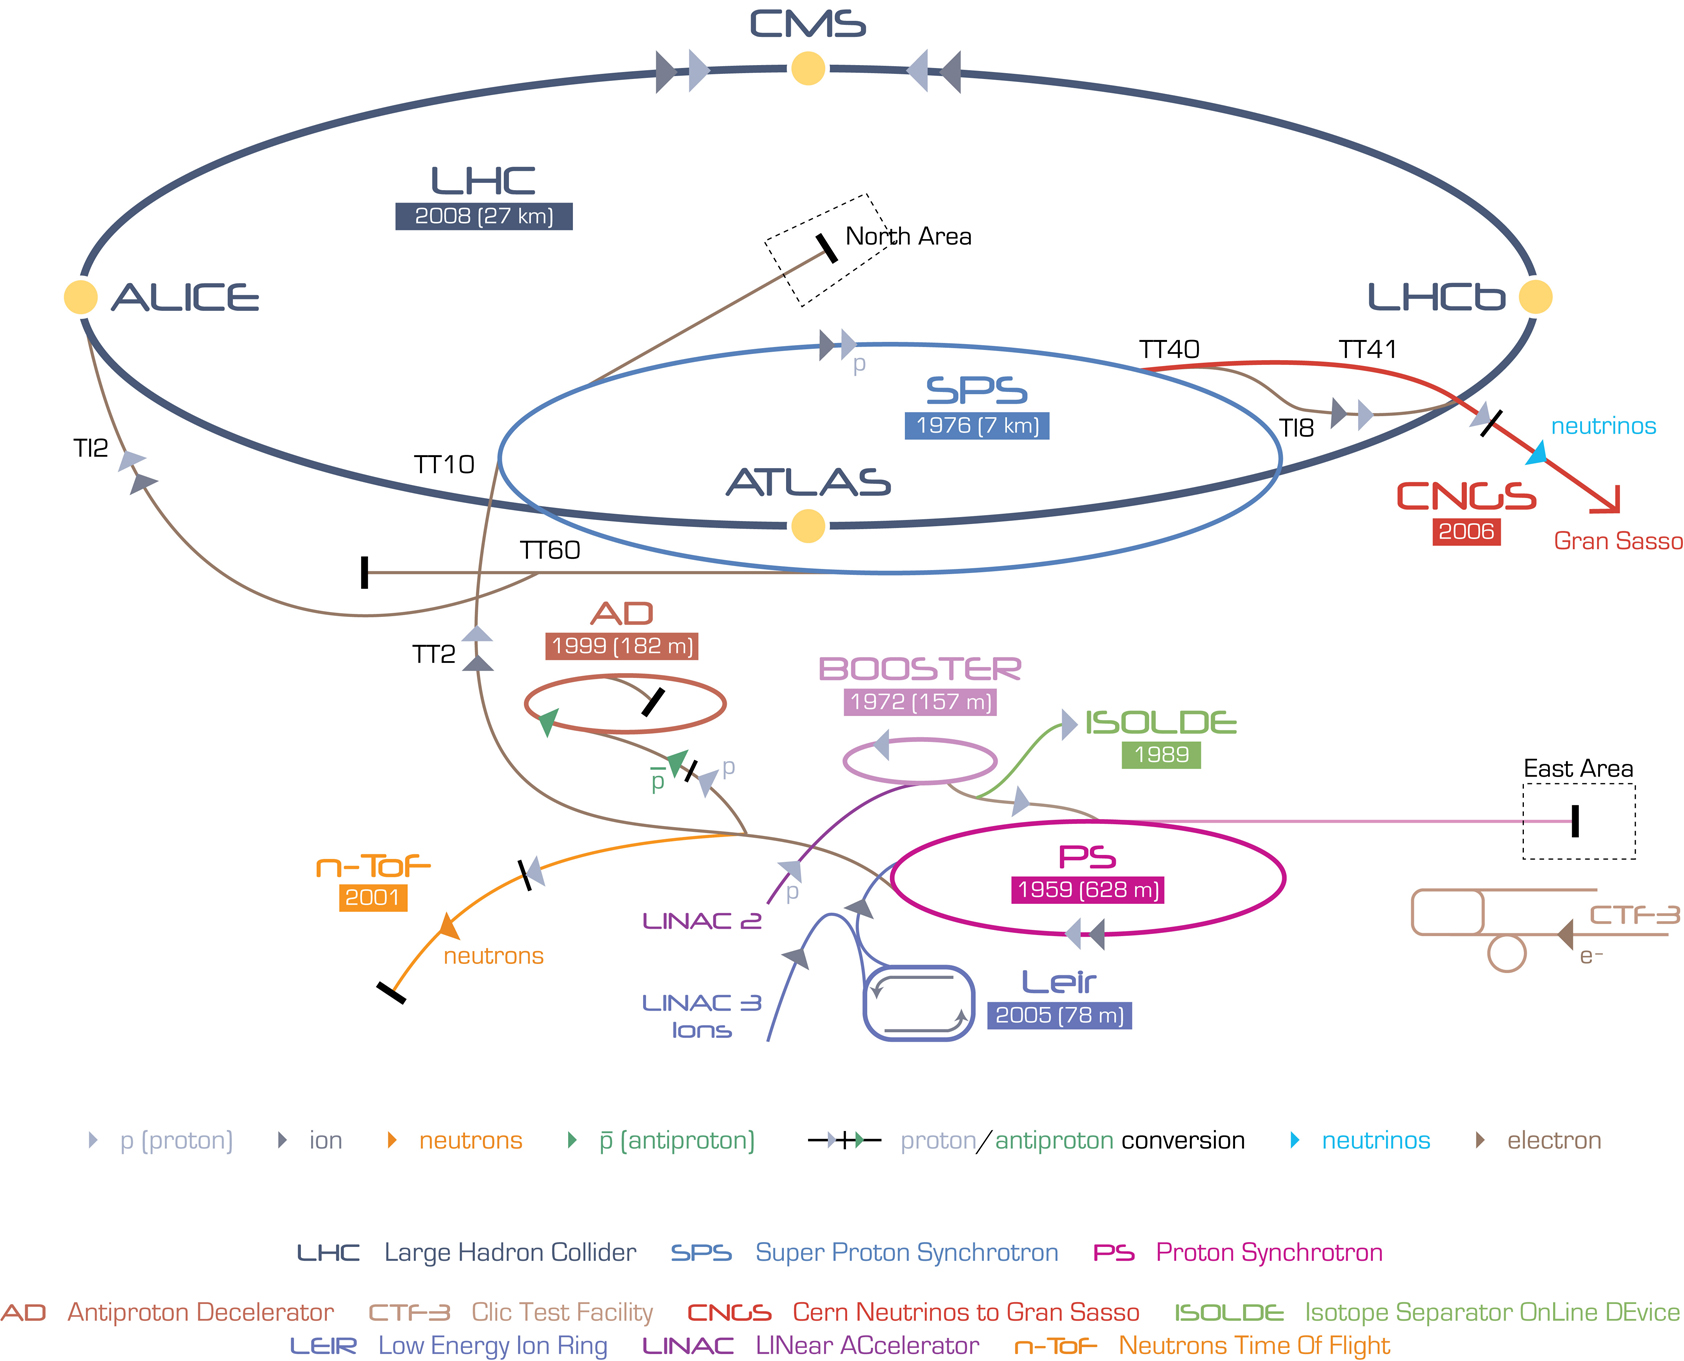
\includegraphics[width=0.6\textwidth]{02_experimental_setup/plots/Cern-Accelerator-Complex.png}
  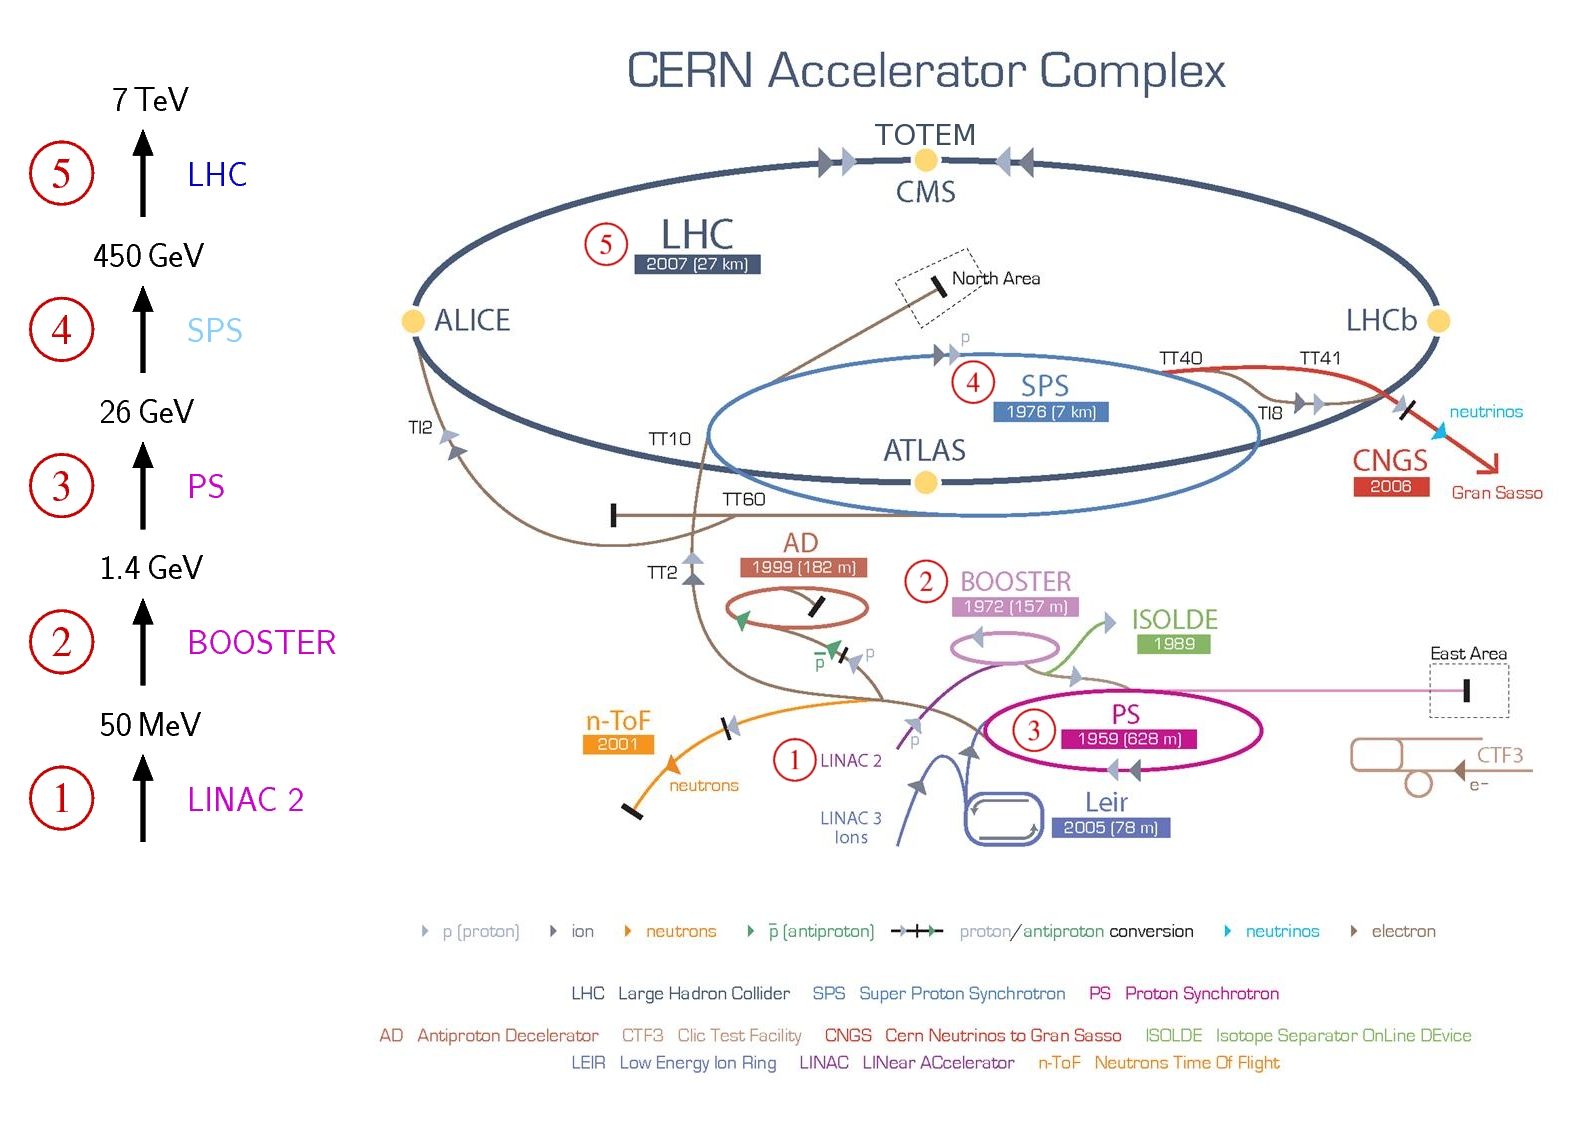
\includegraphics[width=0.8\textwidth]{02_experimental_setup/plots/Cern-Accelerator-Complex-2.png}
  \caption{The complex of accelerators at CERN.}
  \label{fig:AccelCERN}
\end{figure}

\begin{itemize}
 \item[--] Protons first enter the \textit{Linac2} \cite{Arnaudon:1004186} where they are accelerated up to 50 MeV and sent to the Proton Synchrotron Booster (PSB);
 \item[--] \textit{PSB}\cite{Benedikt:2000bs} is composed of four synchrotron rings (to avoid charge repulsion) which raise the energy of the particles to 1.4 GeV
 for injection into the Proton Synchrotron (PS);
 \item[--] \textit{PS}\cite{Benedikt:2000bs} increases the energy up to 26 GeV and it takes 3.6 s to inject the protons to the Super Proton Synchrotron (SPS); 
 \item[--] \textit{SPS}\cite{Benedikt:2000bs} is the second largest accelerator at CERN which provides 450 GeV protons injected to the LHC.
\end{itemize}

The most important accelerator characteristic is the number of protons 
in a coincidence area per time called \textit{instantaneous luminosity} $\mathcal{L}$. The designed value 
at the LHC is $\mathcal{L} = 10^{34}$ cm$^{-2}$ s$^{-1}$. The accelerator was providing $\mathcal{L} = 7.7 \cdot 10^{33}$ cm$^{-2}$ s$^{-1}$
during the run in 2012.

The integral of the instantaneous luminosity over the time
is defined as \textit{integrated luminosity} $L$: 
\begin{equation}\label{eq:lumi}
  L  = \int\mathcal{L}dt.
\end{equation}
LHC provided 23.3 fb$^{-1}$ of integrated luminosity for the run in 2012 from which 21.8 fb$^{-1}$ were
recorded by the Compact Muon Solinoid (CMS) detector (see Fig.\ref{fig:LumiCMS}).

\begin{figure}[t]
  \centering
  %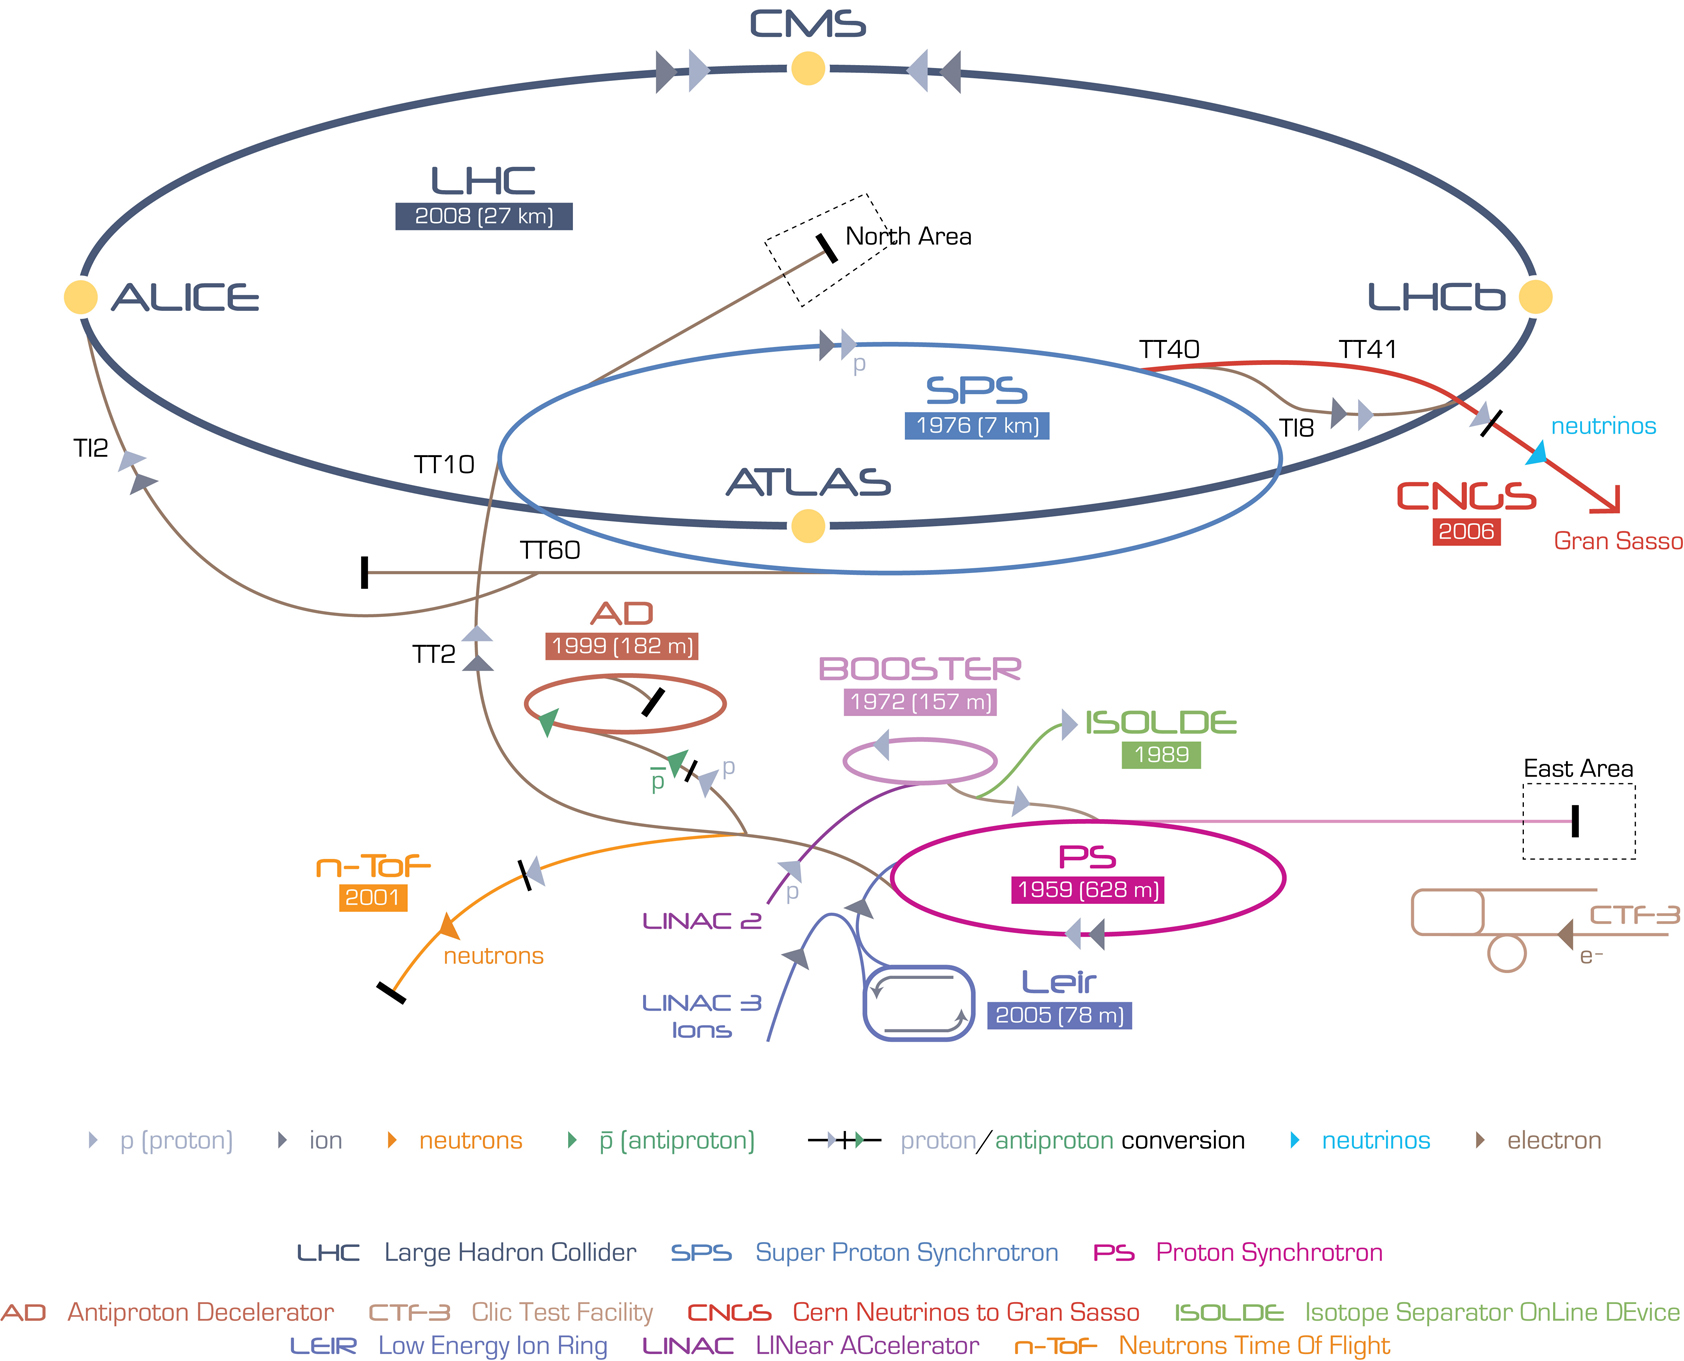
\includegraphics[width=0.6\textwidth]{02_experimental_setup/plots/Cern-Accelerator-Complex.png}
  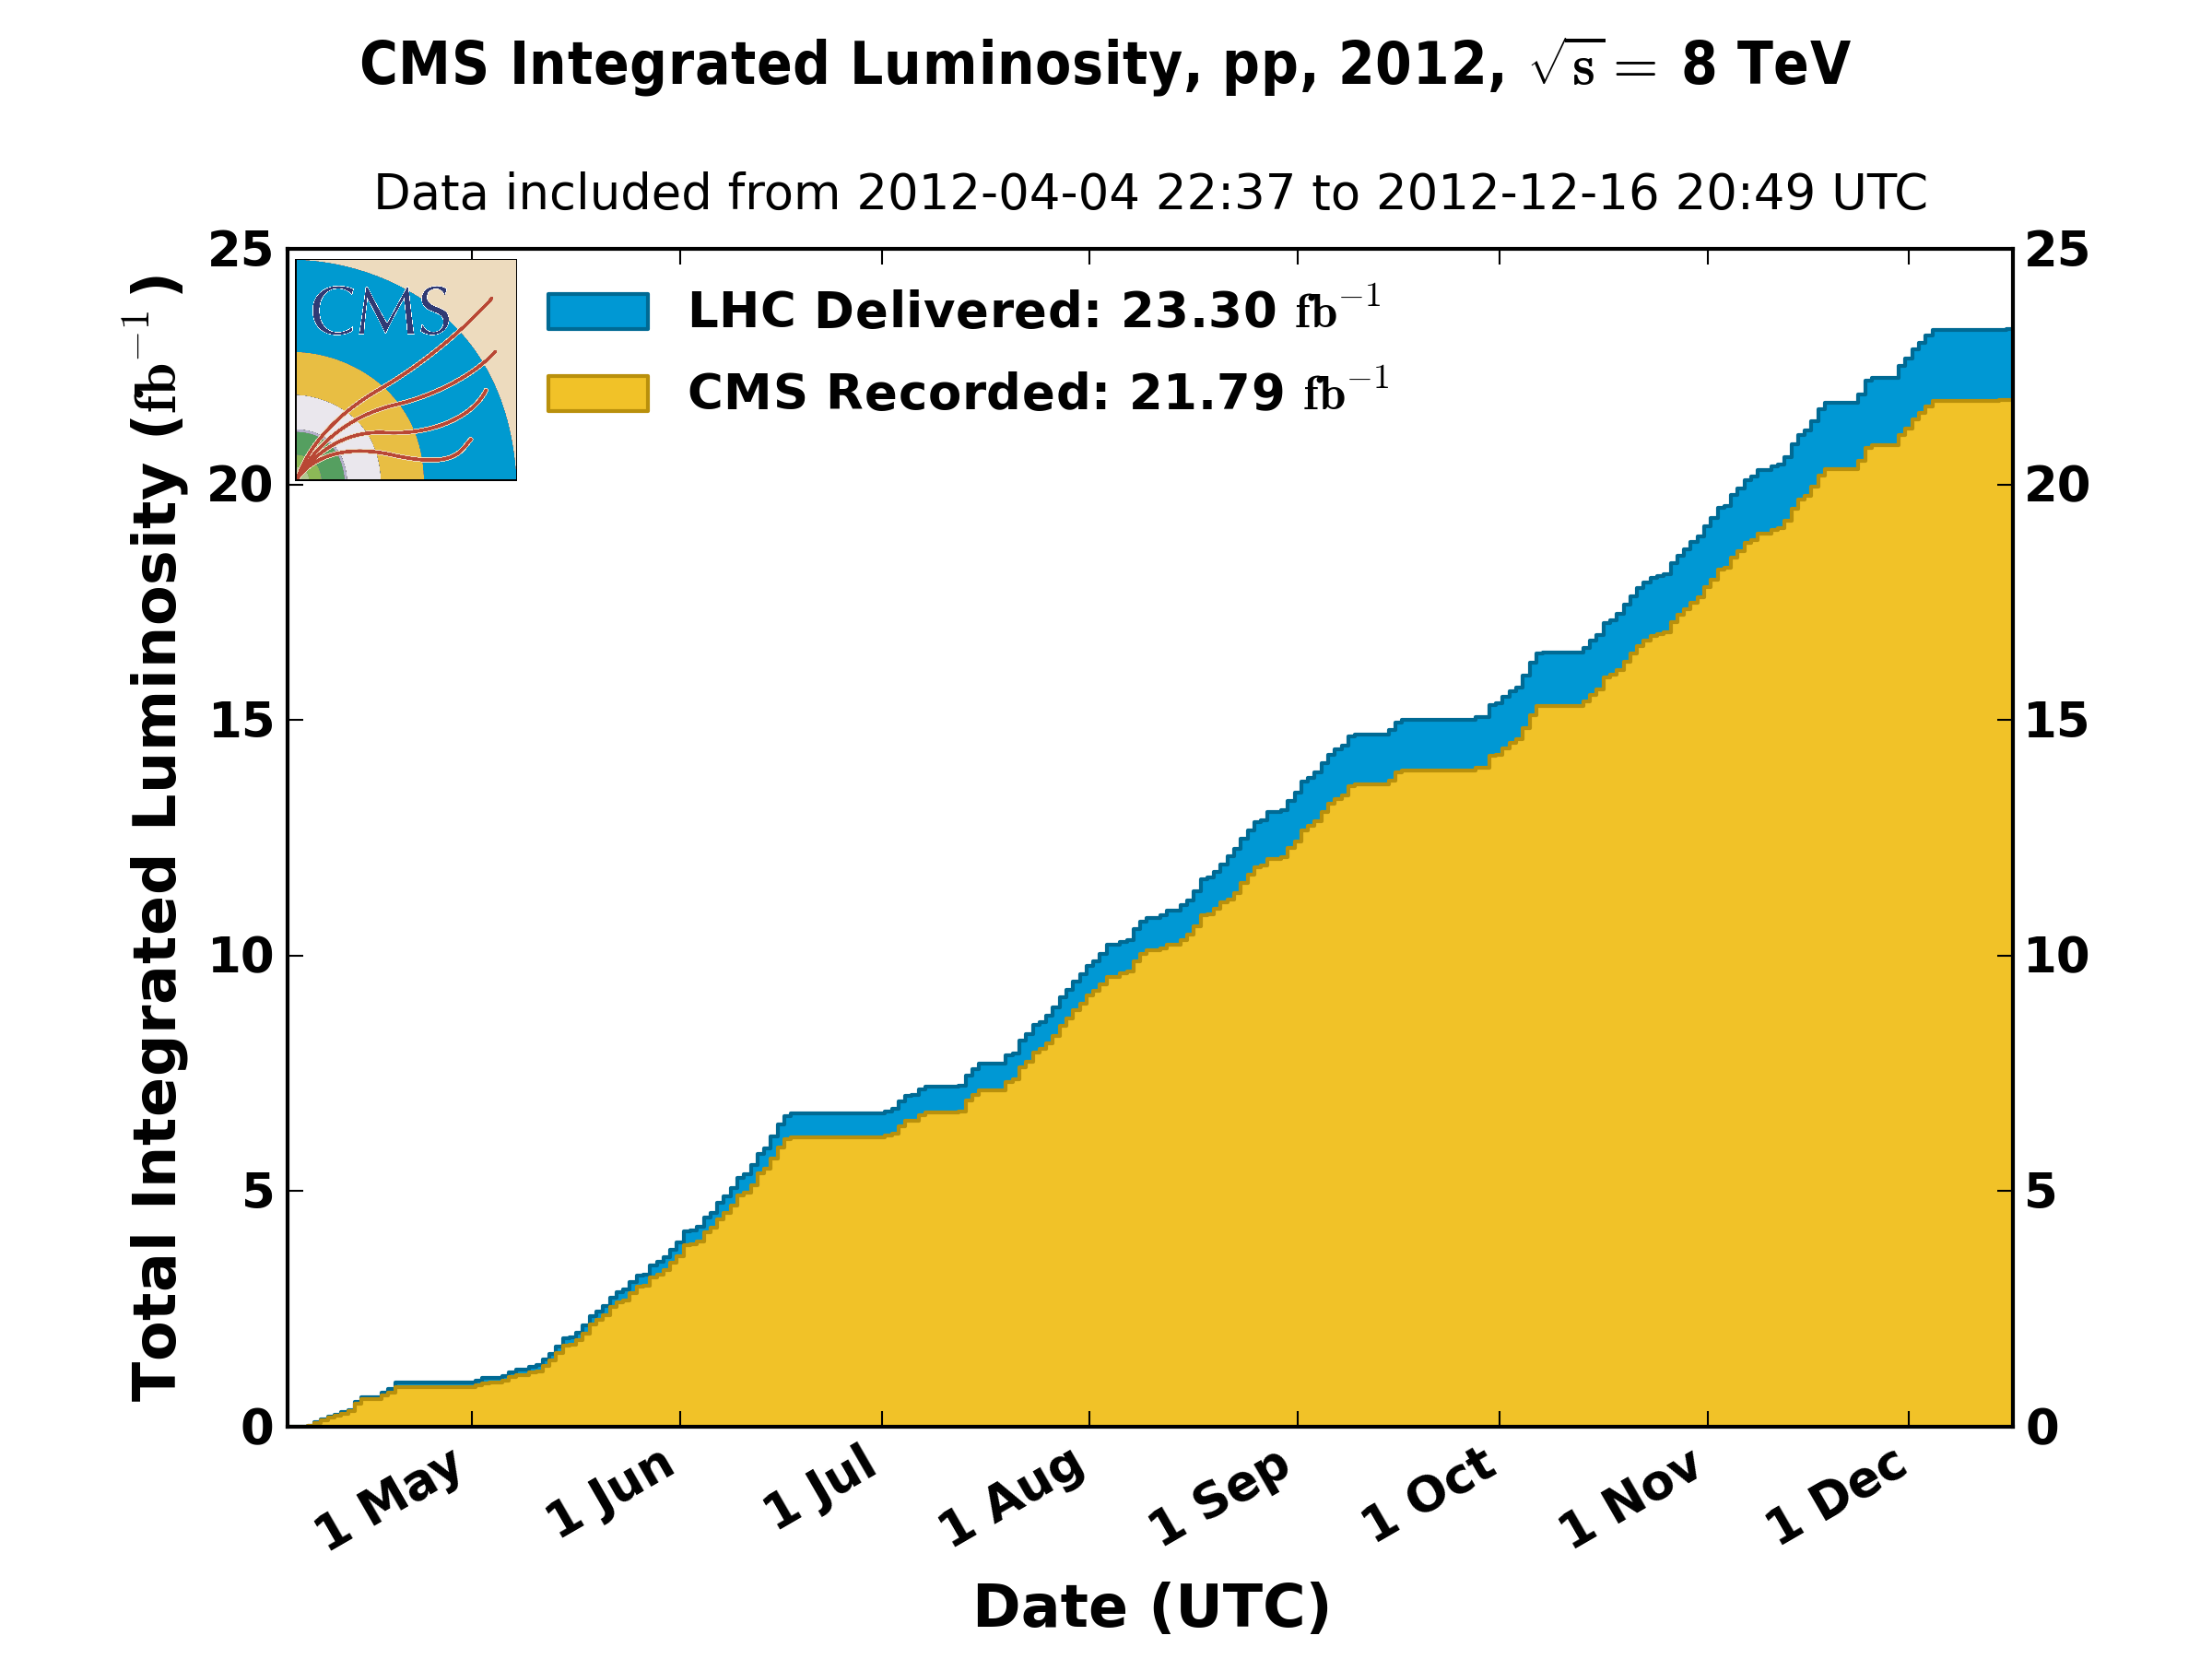
\includegraphics[width=0.6\textwidth]{02_experimental_setup/plots/int_lumi_per_day_cumulative_pp_2012.png}
  \caption{Cumulative luminosity versus day delivered (blue) and recorded by the CMS (orange) for proton-
  proton collisions during stable beam time in 2012.}
  \label{fig:LumiCMS}
\end{figure}

% During the 2012 LHC run period $3.16 \cdot 10^16$[?] protons were delivered which means only ~$1$ mm$^3$ of Hydrogen gas 
% under the normal conditions is needed (taken the efficiency of proton source to account[?]). 

%http://www.lhc-closer.es/1/3/10/0
%https://indico.cern.ch/event/219327/ -- slide 11

The measurements of the collision products are performed with complex particle detectors. There are four of them on the 
LHC ring, \textit{ALICE}, \textit{LHCb}, \textit{ATLAS} and \textit{CMS}, each located around the point where beams 
of particles of different directions are brought to collision.
These detectors have different construction according to slightly different physics goals.

\begin{itemize}
 \item ALICE (A Large Ion Collider Experiment)\cite{ALICEtdr} is designed to
 work with heavy ion collisions. The goal of the ALICE experiment studies is
 the strongly interacting matter in extremely high density state called \textit{quark-gluon plasma}. This 
 state of matter provides a unique possibility to find a bare quark and also to study the early
 Universe which was so dense at the first moments after the Big Bang.
 \\
 The ALICE detector weights 10000 tons and is 26 m long, 16 m high and 16 m wide. It lies on a depth of
 56 m below the ground on the territory of France.
 
 \item LHCb (Large Hadron Collider beauty)\cite{LHCb} is investigating $CP$ violation and heavy flavour physics via
 rare $B$ hadron decays. As the $b\bar{b}$ pairs are mostly produced in the forward and backward directions, 
 and their production cross section is very high, there was no need to construct a big and expensive $4\pi$ detector 
 complex. For this reason the LHCb is a one side spectrometer corresponding to the forward beam direction.
 For a better detection of the $b$-decays the LHCb features a movable tracking system which can go very close
 to the beam pipe.
 \\
 The LHCb detector weights 5600 tons and is 21 m long, 10 m high and 13 m wide. It is located at a depth of 100 m 
 below the ground on the territory of France.
 
 \item ATLAS (A Toroidal LHC ApparatuS)\cite{ATLAS} is one of the two general purpose detectors at the LHC. It serves to reach many physical
 goals -- from Standard Model examination and Higgs searches to the studies of dark matter, extra dimensions and new physics.
 These tasks are mainly similar to the ones from the CMS experiment (the second general purpose detector at the LHC ring), but
 it uses different technical solutions.
 \\
 The ATLAS machine is built around the beam pipe such that the collision point is located in its center. It consists of the 
 inner tracking system and calorimeter, both surrounded by the barrel (2 T) and toroid magnets (0.5 to 1 T). The muon spectrometer
 is located on the outer layers of the detector.
 \\
 Having a length of 45 m, a height of 25 m and a width of 25 m ATLAS is the largest particle detector complex in the world. However, it's mass 
 is rather low reaching 7000 tonnes. It is situated in a cavern 100 m under the ground on the territory of Switzerland.
 
 \item The CMS (Compact Muon Solenoid) is the second general purpose detector on the LHC. A more detailed description of this apparatus will follow in
 section \ref{sec:CMS}.
 
\end{itemize}


% Two much smaller experiments are also located at the LHC ring alongside the four larger ones mentioned above. They are focused on forward particles
% researches which do not collide but rather brush past each other and continue their flow along the beam direction. Thus these facilities do not
% need to be based around the beam coincidence points. The names of the two experiments are \textit{LHCf} and \textit{TOTEM}.

%%%%%%%%%%%%%%%%%%%%%%%%%%%%%%%%%%%%%%
%%%%%%%%%%%%%%%%%%%%%%%%%%%%%%%%%%%%%%
%%%%%%%%%%%%%%%%%%%%%%%%%%%%%%%%%%%%%%
\section{The Compact Muon Solenoid}\label{sec:CMS}

The analysis presented in this work was performed on the data recorded by the Compact Muon Solenoid (CMS) detector\cite{CMSatLHC} during the 2012
run period in proton-proton collisions with center-of-mass energy $\sqrt{s} = $8 TeV. This section will describe in more detail 
the construction and performance of the CMS detector.

Any particle detector is being constructed with respect to the measurements which are planned to be done with it. The main purpose of the CMS detector
is the accurate measurement of the trajectories and momenta of all particles produced in a energetic $p-p$ collision. Different physical
tasks provide special requirements for specific experimental setup parts. If the plan is to measure Standard Model decays
($W$, $H$, $Z'$ decays with leptons in final state), the detector complex has to comprise precise electromagnetic calorimetry and 
muon systems for lepton reconstruction. To measure QCD processes with jets in final states, a
hadronic calorimetry has to provide absolute energy determination with good resolution. To look for heavy resonances one needs a
precise detection in mainly central region, perpendicular to the beam direction, as the low mass resonances fly mostly in the forward
regions, providing backgrounds for the heavy resonances decay products. A particle identification precision relies on a magnet system which bands the charged 
particles differently corresponding to their transverse momentum component and charge. Thus it is important to choose the optimal magnet
shape and power. However, a magnet alone doesn't provide a measurement. To reconstruct precisely the trajectory of the particle in the detector, thus
gain an information about curvature (momentum and charge), a detector has to contain a tracking detector. The latter has to manage not only the momentum
reconstruction, which is crucial for any physical process, but also a precise $b$-identification. $B$ mesons have a relatively long lifetime and are able 
to travel away from the collision point before they decay. The separated from the primary $p-p$ interaction point of the particle decay is called a secondary
vertex. This feature can be utilized to identify $B$-hadrons (for more details see sec. \ref{ssec:bTag}). A precise secondary vertex reconstruction is reached with the help of the silicon
pixels of at least micron resolution. To make the measurement of the missing energy possible, the detector has to possibly cover the whole solid angle
around the collision point.

Taken into account the high luminosities (see Sec.\ref{sec:LHC}) at the LHC,
the detectors have to deal with multiple collisions per bunch crossing - pile up. Not to get distorted by a large amount of particles 
flowing to one sensor unit, the detector must have a fine enough granularity. The designed bunch spacing of 25 ns 
requires a fast enough readout. Radiation hardness of the materials is very important considering high luminosity and small
bunch spacing. In the end the price and feasibility play a crucial role in the detector complex creation.

The CMS facility being a general purpose detector was designed to make it's parts fulfill as many physical goals as possible.
The final onion-like construction of the apparatus is shown in Fig. \ref{fig:CMSview}. The overall detector size reaches 28.7 m in length
and 15.0 m in width. The total weight of the facility is 14000 tones, which makes CMS the heaviest particle detector at the
LHC. The detector is cylindrically symmetric around the beam pipe and also symmetric to the left and right sight along the beam direction
relative to the collision point.

\begin{sidewaysfigure}[p]
  \centering
  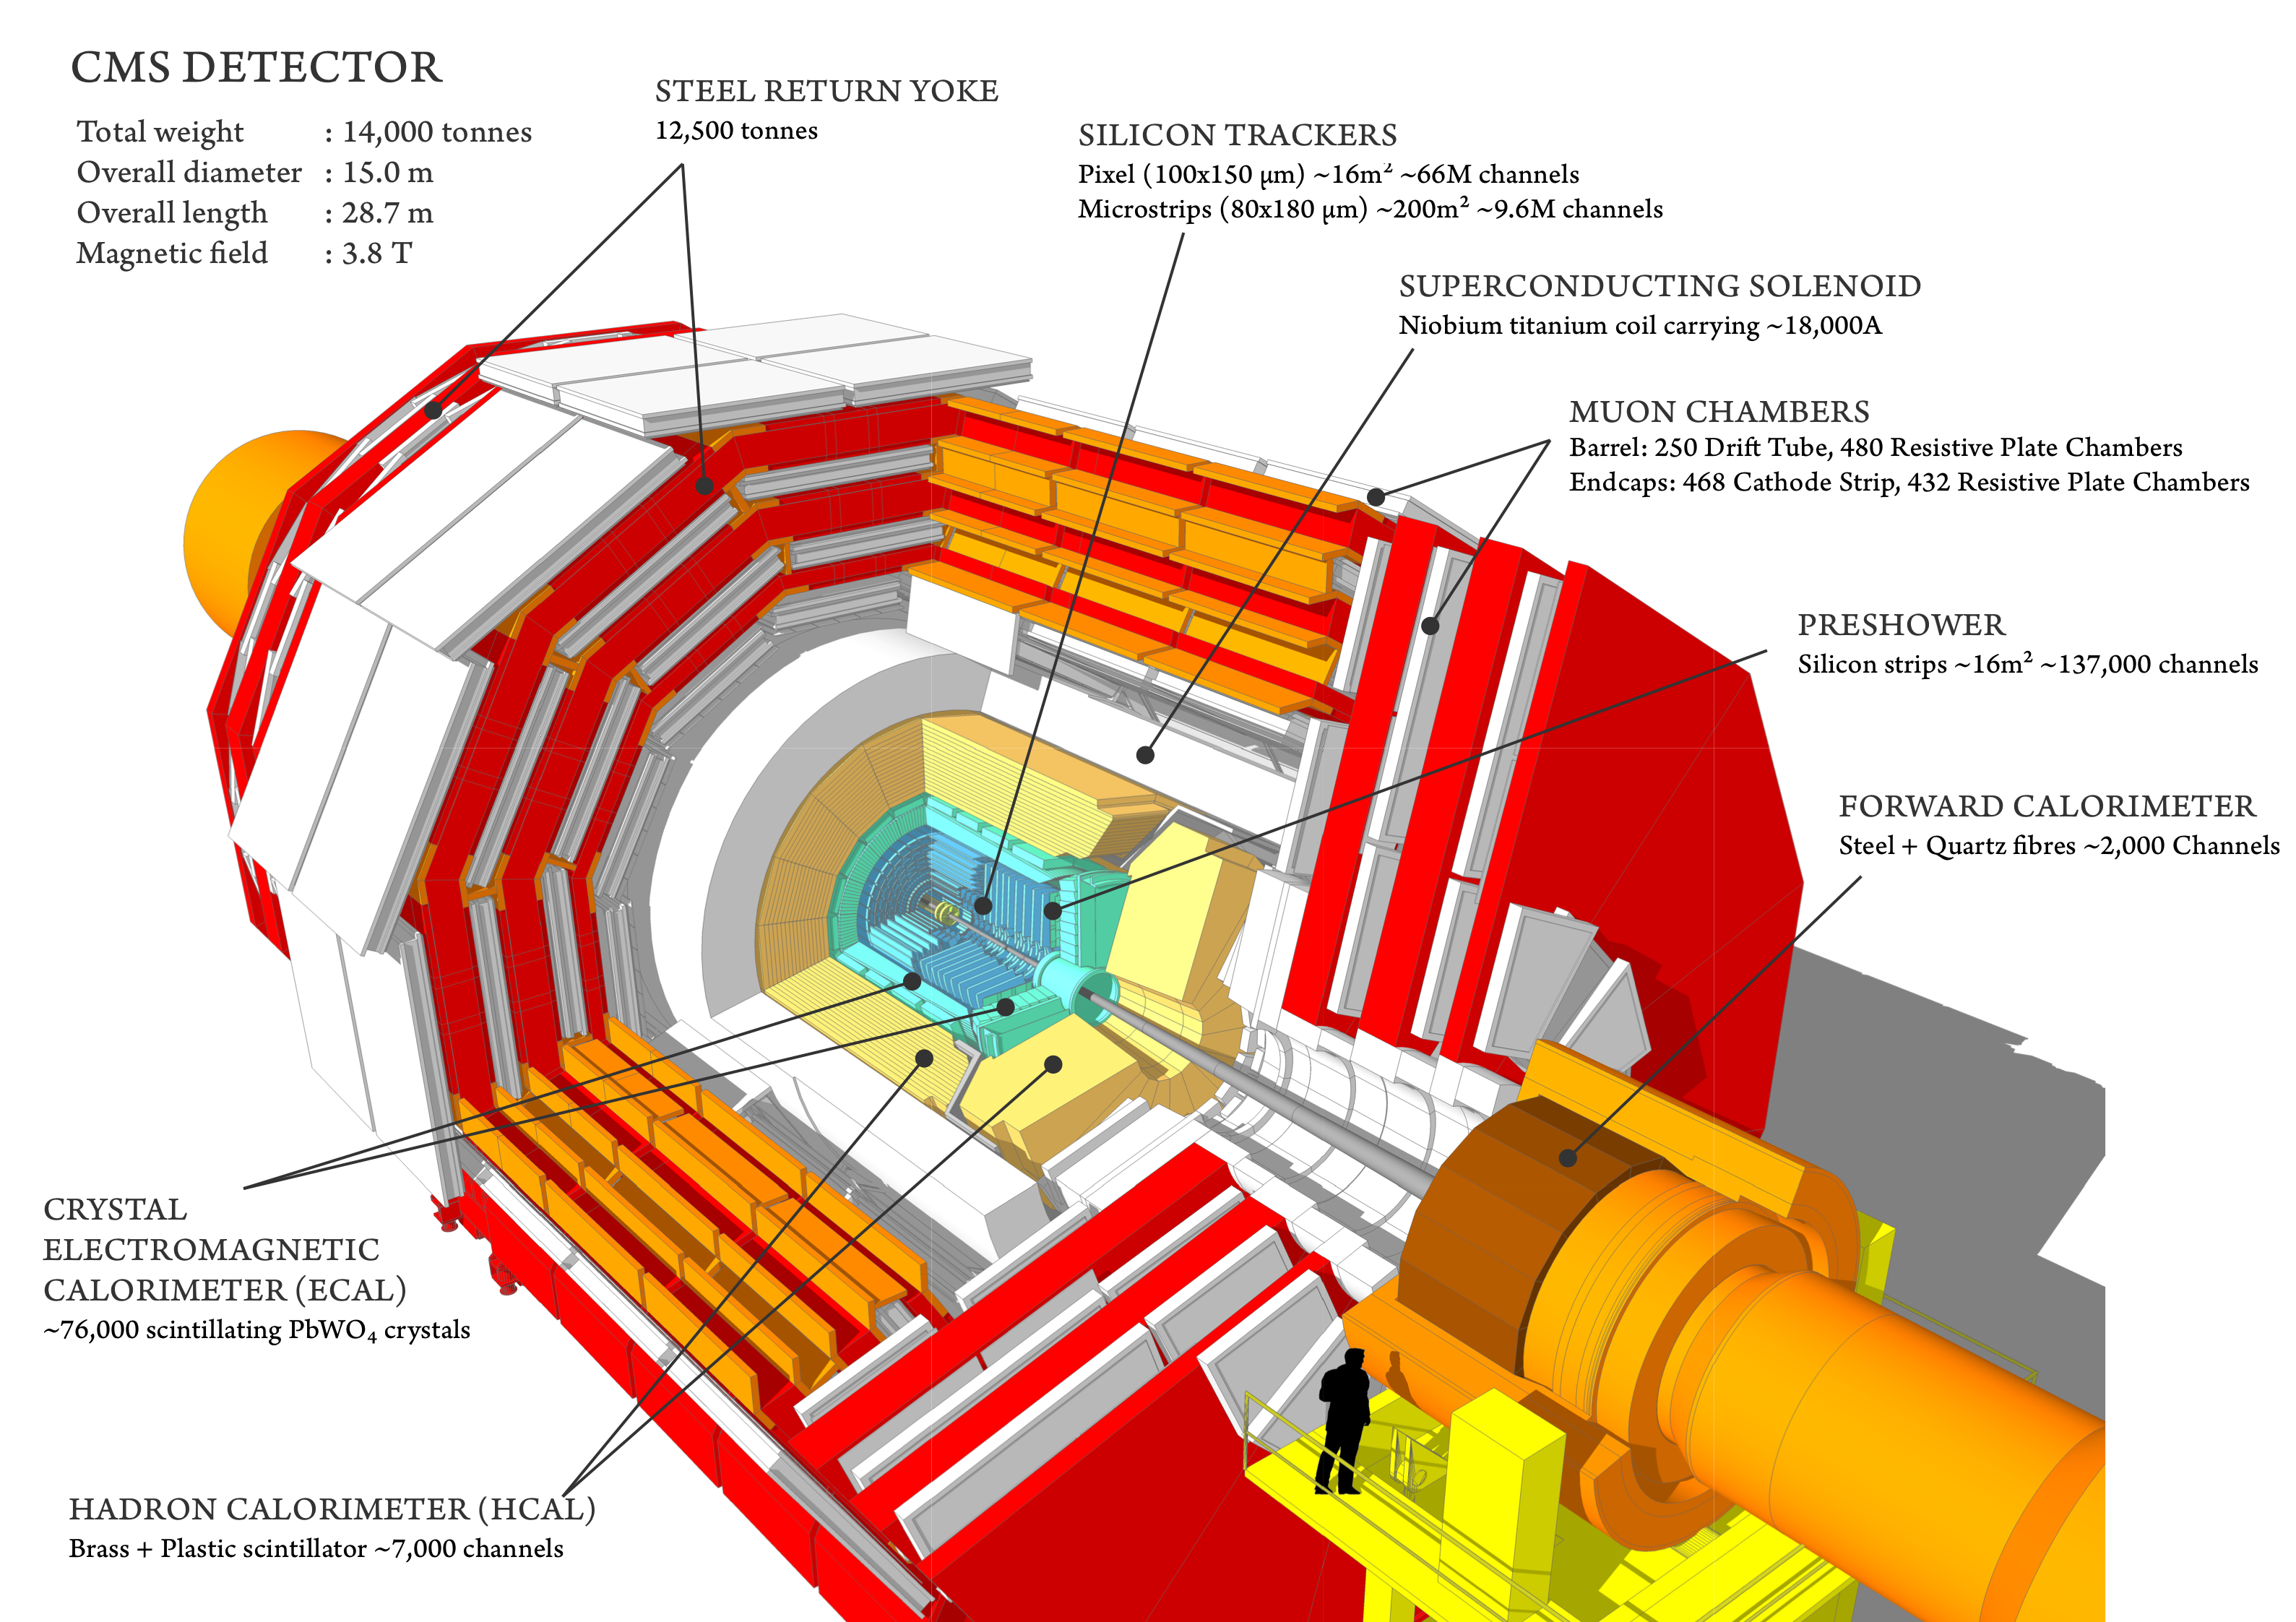
\includegraphics[width=0.8\textwidth]{02_experimental_setup/plots/cms_120918_03.png}
  \caption{Sectional view of the CMS detector with highlighting different components. 
  The LHC beams collide in the center of the machine. The central axis of the detector 
  corresponds to the beam line.}
  \label{fig:CMSview}
\end{sidewaysfigure}

A common coordinate system is used with the CMS experiment. The origin  
is assumed to be located at the nominal collision point, the $x$-axis is pointing to the center of the 
LHC ring and the $y$-axis is pointing vertically upwards. Thus the $z$-axis points along the beam axis to make
the coordinate system right-handed. As the detector is symmetric around the beam pipe, it may be convenient to use cylindrical or spherical
coordinate systems. The azimuthal angle $\phi$ is measured from the $x$-axis in the $x-y$ plane in the range $(0, 2\pi)$ 
and the polar angle $\theta$ from the $+z$-axis in the range $(0, \pi)$. The radial coordinate $r$ is the transverse distance from the coordinate origin. 

The \textit{pseudorapidity} $\eta$ is often used instead of the polar angle:

\begin{equation}\label{eq:eta}
  \eta = -\ln(\tan(\frac{\theta}{2})) = \frac{1}{2}\ln\frac{|\vec{p}| + p_{L}}{|\vec{p}| - p_{L}},
\end{equation}
where $\bar{p}$ is the particle momentum vector and $p_{L}$ is a longitudinal component.
The other variable which can be used instead of $\eta$ for the massive particles is the \textit{rapidity} $y$:

\begin{equation}\label{eq:y}
  y = \frac{1}{2}\ln\frac{E + p_{L}}{E - p_{L}},
\end{equation} 
where $E$ is the energy of the particle.

The transverse momentum and energy of a particle, denoted as $p_{T}$ and $E_T$, are also commonly used in the data analysis. 
They are defined in the $(x-y)$ plane. Another variable representing the energy imbalance in the transverse plane, is the
\textit{missing transverse energy} $E_{T}^{miss}$.

%%%%%%%%%%%%%%%%%%%%%%%%%%%%%%%%%%%%%%
\subsection{Solenoid magnet}\label{ssec:solenoid}

The 3.8 T superconducting CMS solenoid, 13 m in length and 6 m in diameter, is shown in the Fig.\ref{fig:solenoid}. 
The flux is returned through a 10000 ton heavy yoke \cite{CMSatLHC}. A very strong magnet allows not only curving
high momentum muons for their better transverse  momentum reconstruction, but also keeps soft particles with a small bending radius
inside the inner detector layers. This reduces occupancy inside the calorimeters allowing only higher
momentum particles to pass through. A solenoid design allows a compact size of the powerful magnet.
On the other hand this limits the tracking precision at high pseudorapidities, as in the very forward regions there will be 
tracks, which are not influenced by a magnetic field\cite{Dissertori:2010xe} and thus their transverse momentum cannot be measured.


\begin{figure}[t]
  \centering
  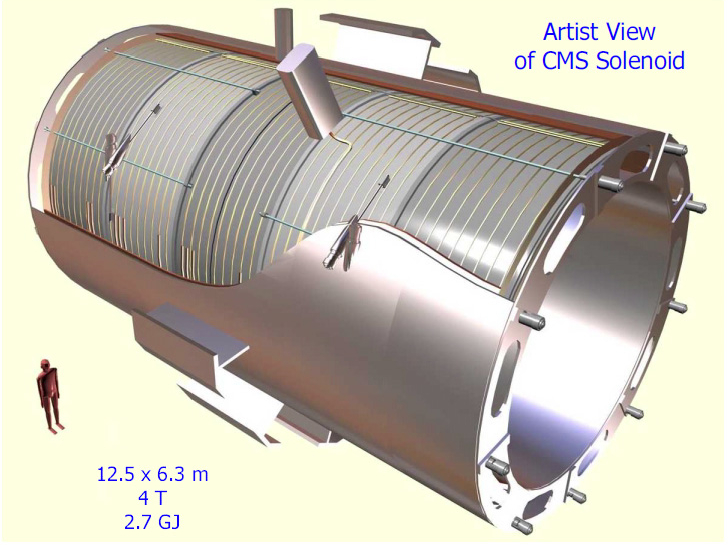
\includegraphics[width=0.6\textwidth]{02_experimental_setup/plots/CERN_CMS_Solenoid_schematic.jpg}
  \caption{The schematic view of the CMS solenoid}
  \label{fig:solenoid}
\end{figure}

%%%%%%%%%%%%%%%%%%%%%%%%%%%%%%%%%%%%%%
\subsection{Tracking Detector}\label{sec:tracker}

The inner tracking detector\cite{TrackerTDR, CMSatLHC} (also called tracker) at CMS is the closest detector component to the beam line and to the collision point having a
length of $5.8\;$m and a diameter of $2.5\;$m. It is designed for a precise track and secondary vertex measurement. 
The tracker is positioned inside the solenoid (see Section \ref{ssec:solenoid}). The particle momentum measurement is the best in the areas where the magnetic field
is sizable. This corresponds to the central pseudorapidity ranges $|\eta| < 2.5$ thus the most emphasis of the tracker design is on the central
areas. The requirements of high granularity, fast readout and radiation hardness lead to a tracker design based entirely on silicon
detectors technologies. The tracking detector consists of \textit{pixel} and \textit{strip} silicon modules
and its overall structure is displayed in Fig.\ref{fig:tracker}.

\begin{itemize}
 \item The pixel detector is located at the closest distance to the proton-proton collision point. It is composed of three co-axial barrel layers (BPIX)
 4.4 cm, 7.3 cm and 10.2 cm far from the beamline and two forward discs (FPIX) on positive and negative z sides
 at $\pm$34.5 cm and $\pm$46.5 cm. Altogether the detector consists of 66 million pixels each of a size $100 \times 150\;\mu$m$^2$. A hit
 position resolution of 15-20 $\mu$m was reached\cite{TrackPerf}.
 As shown in Fig.\ref{fig:tracker}, the pixel detector covers the rapidity range $|\eta| < 2.5$.
 
 \item A silicon strip detector composed of ten layers follows right after the pixel detector and reaches a distance of 130 cm far
 from the beamline. It consists of four inner barrel layers or Tracker Inner Barrel (TIB), two inner endcaps each containing 3 discs
 or Tracker Inner Disk (TID), six outer barrel layers or Tracker Outer Barrel (TOB) and two outer Tracker EndCaps (TEC).
 Each of the components has a specific design corresponding to it's position. The sensors in TIB and TOB are placed parallel to the
 beamline, and in TID and TEC they are perpendicular to the beam pipe. Overall the silicon tracker consists of 9.3
 million strips.
\end{itemize}

\begin{figure}[t]
  \centering
  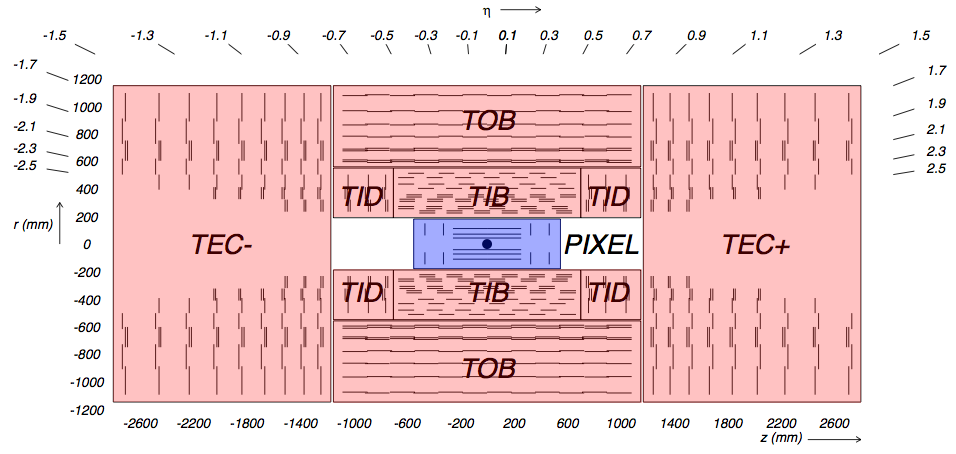
\includegraphics[width=1.1\textwidth]{02_experimental_setup/plots/img_cms_tracker_view.png}
  \caption{CMS tracking detector. The pixel part is marked with blue and the strip part is marked with red.}
  \label{fig:tracker}
\end{figure}

With overall 200 m$^2$ of active silicon area CMS tracking detector became the largest silicon tracker ever built. 

%%%%%%%%%%%%%%%%%%%%%%%%%%%%%%%%%%%%%%
\subsection{Electromagnetic Calorimeter}

The Electromagnetic Calorimeter (ECAL)~\cite{ECALtdr, ECALtdradd, CMSatLHC} is a detector component which comes next after the tracker on the way of particles from
the collision point. The facility is assigned to measure the full electron and photon energies in all the directions. 
A very special lead tungsten (PbWO$_{4}$) scintillating crystal was made to build up the ECAL. The crystalline is heavier then stainless steel but transparent. 
Each crystal weights 1.5 kg having a size from $22\times22\;$mm$^2$ to $26\times26\;$mm$^2$ with the length of 230 .

The ECAL is a homogeneous detector made up of the \textit{barrel} part (EB) covering the range of $|\eta| <$ 1.479 and two \textit{endcaps} (EE) in the range $(1.479 < |\eta| < 3.0)$
as shown in Fig.\ref{fig:ecal}. For a high precision measurements of the low momentum gamma quanta a \textit{Preshower} is installed right before 
the endcaps.

\begin{figure}[t]
  \centering
  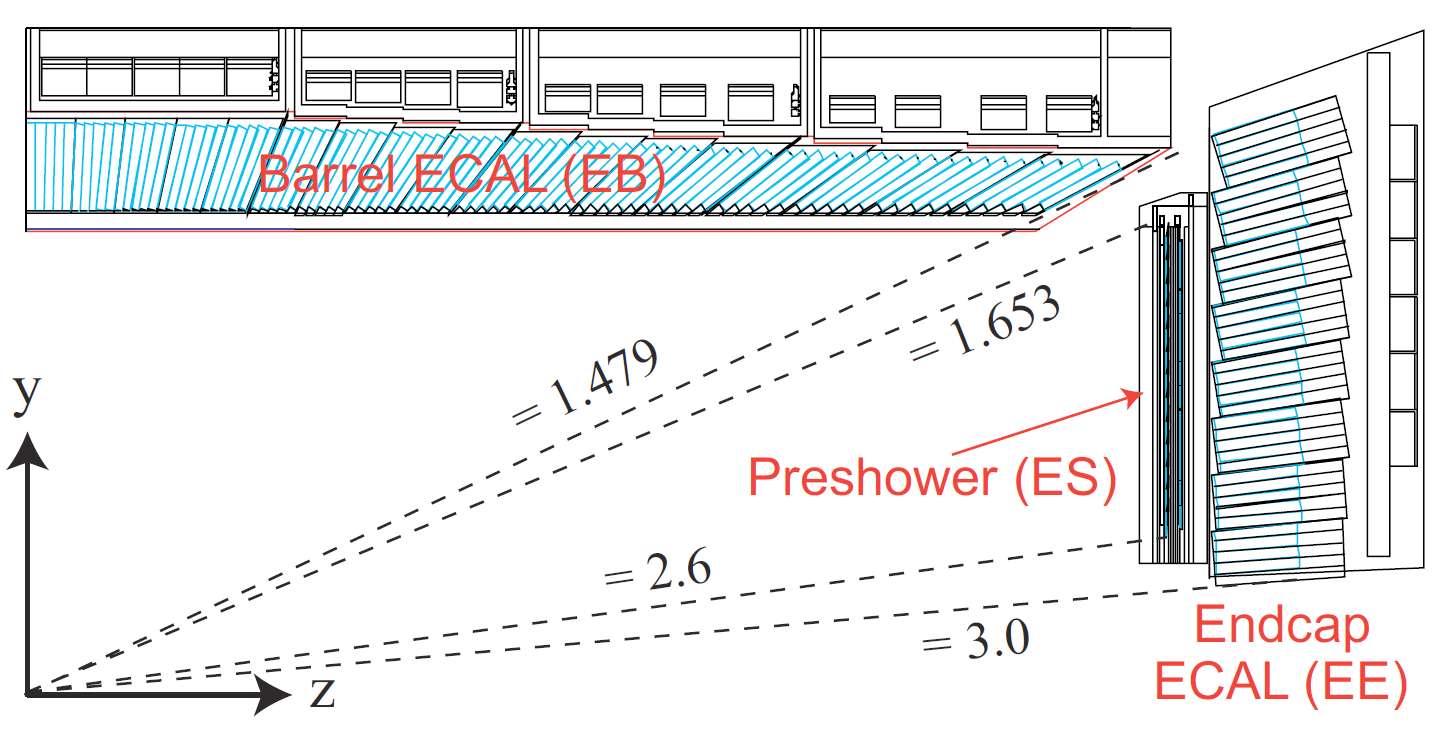
\includegraphics[width=0.8\textwidth]{02_experimental_setup/plots/Figures_Experimental_Apparatus_ECALRapidity.png}
  \caption{CMS electomagnetic calorimeter sketch. Different components and their pseudorapidity ranges are shown.}
  \label{fig:ecal}
\end{figure}

The EB consists of 61200 crystals of lead tungsten joined in modules with 5 crystals in each. It is
cylindrically surrounding the beam pipe starting at a distance of $r = 1.29\;$m from it. 
The material is dense and thus reduces the particle's path allowing a smaller overall size of this detector component. 
Each crystal has a length of 230 mm, corresponding to 25.8$X_{0}$\footnote{The radiation length in PbWO$_{4}$ is 
$X_{0}=0.86$ cm. It corresponds to the distance which an electron should pass in this specific material to reduce it's 
energy by a factor of $\frac{1}{e}$ and to $\frac{7}{9}$ of the mean free paths for a pair production by a photon.}. 
To avoid the particles traveling through the cracks between the single submodules they are all tilted by 3$^{\circ}$ with 
respect to the direction to the nominal collision point. The lead tungsten scintillation decay time\footnote{The scintillation decay 
time is the time required for scintillation emission to decrease to $e^{-1}$ of its maximum.} is of the order of 25 ns, thus 80$\%$ 
of the light signals are emitted fast enough to fit into the bunch spacing designed for the LHC. A special avalanche 
photomultiplier designed to work under the high magnetic fields is glued on the back side of each crystal to detect the scintillated light\cite{APDVPT}.

A Preshower forms a 20 cm thick disc which contains two layers of lead to form the showering each followed by a layer of silicon strips to
detect the particles from the shower. A much finer granularity of the silicon strips (2 mm wide each) compared to the 
crystals in EB and EE allow a more accurate particle distinction.

The EE consists of two endcups each being composed of 7324 lead tungsten crystals placed at $z = \pm 3.154\;$m. As for the EB the modules
at EE are slightly tilted but each crystal is a bit shorter compared to the barrel layer (24.7$X_{0}$). Vacuum phototriodes\cite{APDVPT} were
glued to the back side of the scintillating planes.

The energy resolution $\sigma(E)$ of the ECAL detector is given as\cite{CMSatLHC}:

\begin{equation}\label{eq:resECAL}
  (\frac{\sigma}{E})^{2} = (\frac{S}{\sqrt{E}})^{2} + (\frac{N}{E})^{2} + C^{2},
\end{equation} 

where $S$ is a stochastic term due to measurement fluctuations, $N$ is a noise term due to electronics and pile up noise
and $C$ is a constant term due to systematic imperfections and from temperature instabilities. 
The ECAL energy resolution was primary determined on a test beam using 
electrons in the energy range from 20 GeV to 240 GeV\cite{ECALres2007} and the result was the following:

\begin{equation}\label{eq:resECAL}
  (\frac{\sigma}{E})^{2} = (\frac{2.8\%}{\sqrt{E}})^{2} + (\frac{12\%}{E})^{2} + (0.3\%)^{2},
\end{equation}

where the variation terms correspond to the ones listed in \ref{eq:resECAL}.

After a measurement of the ECAL characteristics with proton-proton collisions with a centre-of-mass energy $\sqrt{s} = $7 TeV
at the LHC in 2010 and 2011 it was found that for the 60 GeV electrons the energy resolution varies from 1.1$\%$ in the barrel 
to 5$\%$ in the forward regions\cite{ECALres2013}.

%%%%%%%%%%%%%%%%%%%%%%%%%%%%%%%%%%%%%%
\subsection{Hadron Calorimeter}

The Hadron Calorimeter (HCAL)\cite{CMSatLHC} at CMS follows the ECAL and aims to capture until full stop all the particles which entered it, 
except for the muons and the invisible neutrinos. As it is assumed that electrons are absorbed in the ECAL, the HCAL is primarily designed 
to measure the full energy of hadrons. Due to the hermiticity, the detector should identify all hadron decay products in a hard proton-proton
collision. Thus any energy imbalance would point to the existence of non-interacting neutral particles such as neutrinos.

One of the main challenges of the hadronic calorimeter design was to fit it inside the compact solenoid (see sec.\ref{ssec:solenoid}).
The solution was to put one of the parts of the detector component outside the magnet coil. Thus the HCAL consists of the barrel (HB), 
outer barrel (HO), endcup (HE) and forward (HF) parts. A schematic sketch of the hadron calotimeter is presented in Fig.\ref{fig:hcal}.

\begin{figure}[t]
  \centering
  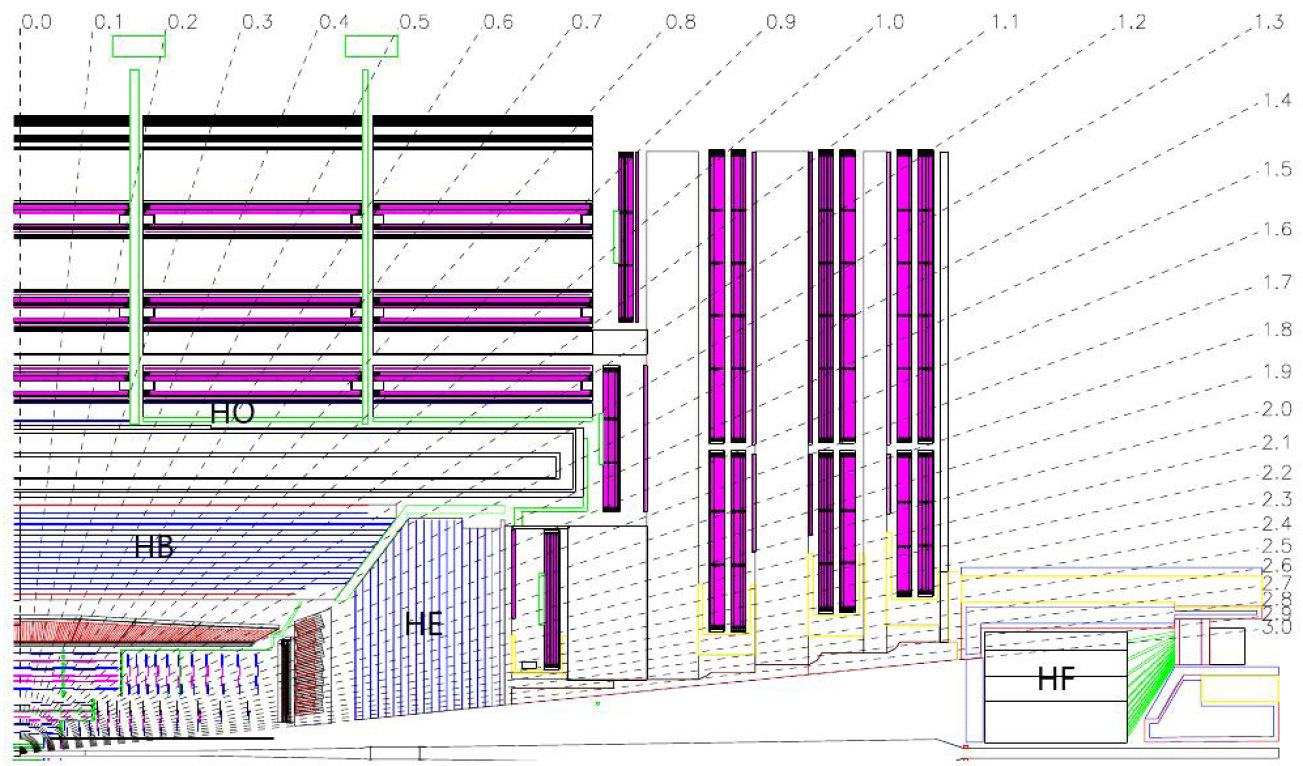
\includegraphics[width=1.0\textwidth]{02_experimental_setup/plots/Figures_Experimental_Apparatus_HCAL.png}
  \caption{CMS hadron calorimeter sketch. Different components and their pseudorapidity ranges are shown.}
  \label{fig:hcal}
\end{figure}

The HB and HE are the sampling calorimeters composed of brass and stainless steel plates (some of them made of Russian Navy brass 
shell casements in World War II) interleaved with scintillators. The HB covers the pseudorapidity range of $|\eta| < $1.3. It contains 14 brass and
2 stainless steel absorbers, each from 50.4 mm to 56.6 mm thick. The HE covers more forward region in pseudorapidity -- 1.6$ < |\eta| < $3.0. It is composed
of 18 layers of 79 mm thick brass plates. The scintillator plastic tiles are located after each absorber layer. The gaps between tiles are covered 
with reflective paint to prevent the light emitted inside one scintillator plate traveling outside as this light gives the energy estimate. Optic fibers fitted into
specially cut grooves on top of scintillating tiles collect light signals and pass them to the readout boxes with hybrid photodiodes. The signals
collected from successive tiles, one behind the other, are optically added and form so called ``towers``. The towers are indicating 
the particle path in the calorimeter.

The HB and HE material thickness provides only 5.82$\lambda_{I}\;\;$\footnote{$\lambda_{I}$ is \textit{nuclear interaction length}, or the average 
length the particle has to travel inside the material before undergoing an inelastic nuclear interaction} in the central region to 10.6$\lambda_{I}$ in the more forward
region. The ECAL material overall is equal to 1.1$\lambda_{I}$. This is not enough to stop all the hadron showers\footnote{To fully contain a 1 TeV hadronic jet a thickness of
roughly 11$\lambda_{I}$.} so the additional outer calorimeter HO
was placed outside the solenoid. Using the solenoid and yoke material itself, adding also some own absorber plates, HO provides additional 11.6$\lambda_{I}$ in the
most central regions.

The forward calorimeter part HF starts at $z = \pm$11.6 m and cover a pseudorapidity range  3.0 $ < |\eta| < $ 5.2. It has a cylindrical shape
with the inner radius $r = $12.5 cm and outer radius $r = $130.0 cm. The overall length of HF is 165 cm. It consists of absorbing steel grooved plates and
quartz light emitting tubes placed in these grooves parallel to the beam pipe. As the HF faces not only hadronic but also the electromagnetic radiation
it has to be sensitive to both. Thus half of the quartz tubes spread over the whole length of the HF (165 cm) and the other half (short quartz tubes) starts only at 22 cm 
from the front side of the HF. The long and the short quartz fibers have different readouts. Electromagnetic showers would start very early  not reaching the 
short quartz tubes.

%%%%%%%%%%%%%%%%%%%%%%%%%%%%%%%%%%%%%%
\subsection{Muon Detector}\label{ssec:muonDet}

The Muon Detector\cite{CMSatLHC} together with the solenoid are the detectors which were giving the name to the CMS detector. As muons pass through calorimeters materials
without significant losses\cite{MuonStop}, the muon detection systems can be placed on the outer layers of the whole CMS apparatus.
The unique signature of a muon in the event can be used for triggering. Muons appear in many processes
of physical interest at CMS, like Higgs or heavy resonances decays.

The muon system stations are located outside the solenoid and in-between the return yoke plates. A muon track is fitted to the hits in each station 
and interpolated to the tracker. That is why the muon system and the central tracking detector have to be aligned with a precision of one sixth of a millimeter.

The muon detector consists of 1400 gaseous chambers of three types: 250 Drift Tubes (DT), located in barrel region of $|\eta| < $1.2, 540 Cathode Strip Chambers
(CSC) as endcaps covering the pseudorapidity of 0.9$ < |\eta| < $2.4 and 610 Resistive Plate Chambers (RPC) placed in both, barrel and endcup regions, and covering
the range $|\eta| < $1.6. A schematic view of the muon detecting system with its components is presented on Fig.\ref{fig:muond}.

\begin{figure}[t]
  \centering
  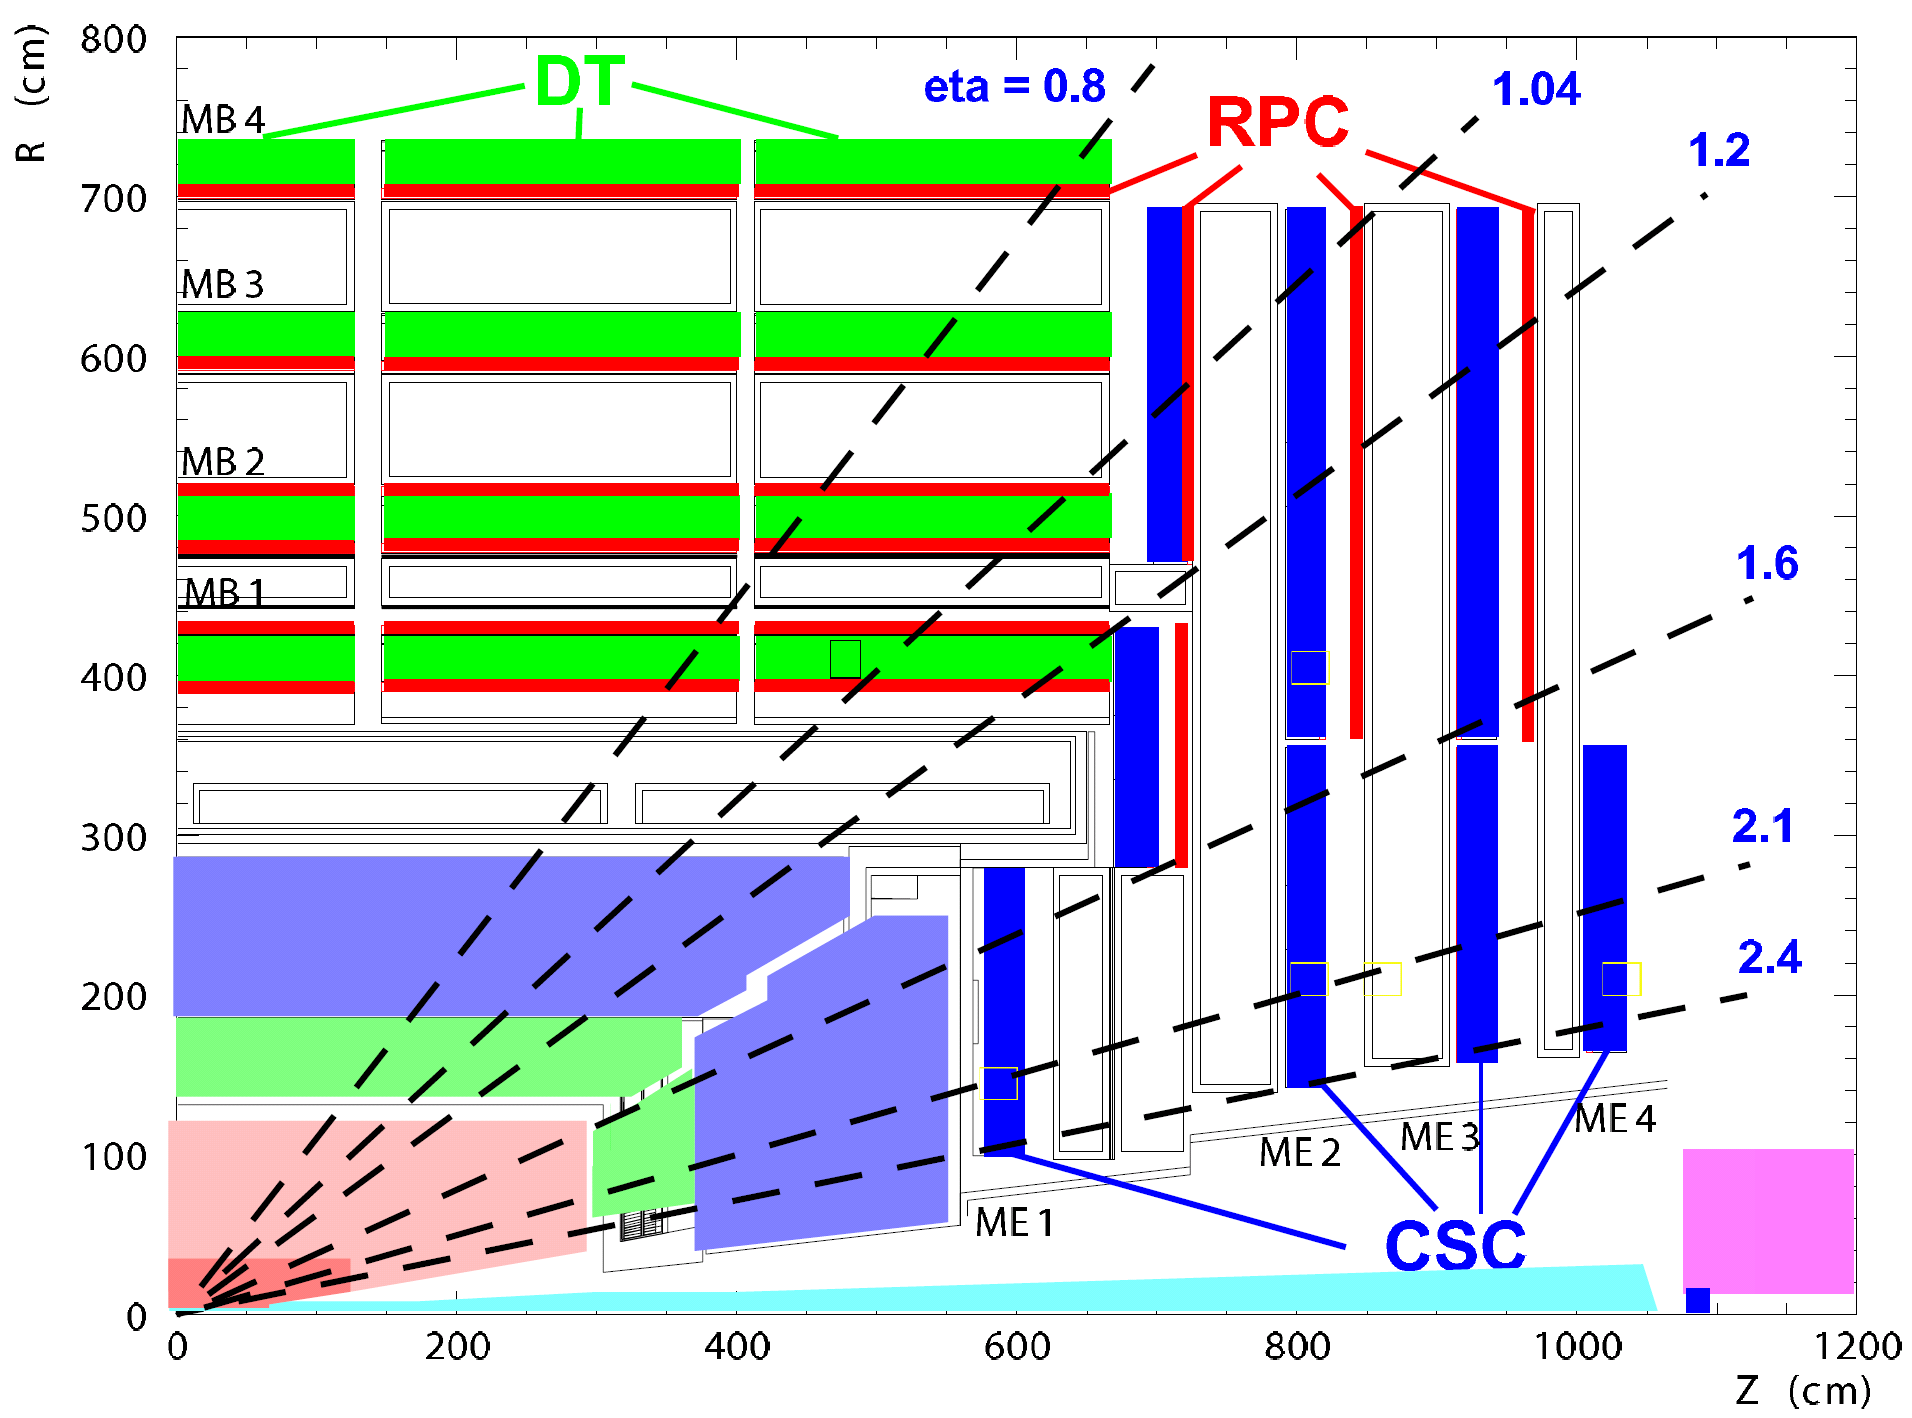
\includegraphics[width=1.0\textwidth]{02_experimental_setup/plots/Figures_Experimental_Apparatus_MuonDetector.png}
  \caption{CMS muon detection system sketch. Different components and their position are shown.}
  \label{fig:muond}
\end{figure}

The DT measures the muon position with a help of a system of 4 cm wide gas tubes filled with 15$\%$ of Argon and 85$\%$ of carbon dioxide.
Each tube contains a stretched positively charged wire inside to collect the charge from the gas ionized by the muons. The DT has four layers
divided into four stations (together with RPCs) each. The stations are aligned parallel to the beam line and measure the coordinates in $(r,\phi)$
plane. Three inner stations additionally provide the measurements in the $z$ direction with four additional radial aligned DTs.

The CSCs disks are used in the endcup regions. Each of them is composed of seven copper cathode strip planes with six anode wire planes in-between, located in 
a gas volume. Wires and planes have perpendicular directions, thus providing two coordinates of the tracks.

The RPCs provide precise timing measurements and can tag from which bunch crossing the particle comes. This is used to trigger (see sec. \ref{sec:trig})
the events.

Muon momentum measurements from a combination of measurements in the muon system and the tracker reach relative resolution of 1$\%$ -- 3$\%$ for muon $p_{T}$
ranging from 20 GeV to 100 GeV.

%%%%%%%%%%%%%%%%%%%%%%%%%%%%%%%%%%%%%%
\subsection{Triggers}\label{sec:trig}

The LHC provides proton-proton collisions every 25 ns, which means that particles from one bunch crossing still travel in the detector at 
the time when the next collision takes place. There is no way to store the huge amount of information from every collision, but even if it were,
a greater part of the events would contain no traces of new physics. Most of the collisions are low energetic with no chance
to produce heavy resonances or Higgs bosons.

Thus there is a need to filter the collisions and record only those which have interesting outcome products. This task is taken over by a trigger
system\cite{CMSatLHC}. Unlike the three-level trigger system commonly used by other collider experiments, CMS has decided to install a first and a high
level trigger omitting the second one.

The \textit{Level-1 trigger} (L1) consists of a custom designed programmable electronics, FPGA, ASICs and programmable look-up tables (LUTs).
The trigger L1 is designed to reduce the nominal LHC collision rate of 40 MHz to 100 kHz. The data from different detector parts is stored
synchronously in a pipeline with a time stamp corresponding to the bunch crossing it appeared from. The information from calorimeters and muon systems is taken to run very primitive
and fast algorithms of particles and jets reconstruction. The information is subsequently collected, compared and is accepted if the trigger
requirements are fulfilled. A more detailed L1 trigger architecture is shown in Figure. \ref{fig:trigA}. The time of the L1 decision is 3.2 $\mu$s. 

\begin{figure}[t]
  \centering
  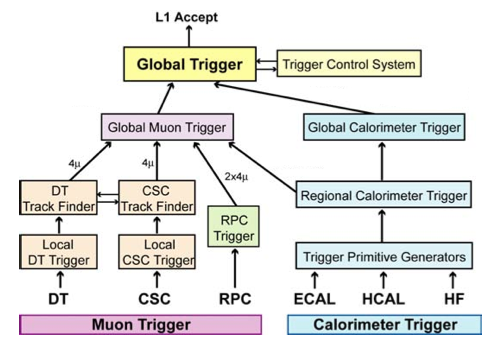
\includegraphics[width=0.6\textwidth]{02_experimental_setup/plots/img_l1.png}
  \caption{CMS Level 1 trigger architecture. The plot is taken from \cite{CMSatLHC}.}
  \label{fig:trigA}
\end{figure}

The \textit{High Level Trigger} (HLT) is a software system represented by a filter farm with about a thousand commercial processors. The information
from the L1 trigger is passed to the computers where it is processed in parallel. The amount of information and readout speed define the requirements
on the transfer network. Complex modern network switches solved these problems. HLT performs a mini-reconstruction of the objects detected,
typically it takes events with leptons, muons and jets with minimum $p_{T}$ and $\eta$ requirement, but also some restrictions on global
event characteristics, like the missing transverse energy $E^{miss_{T}}$ can be set. An event is written if it is accepted by at least one HLT.
If a trigger has a rather low threshold for some physical interest thus accepting too many events, it is being prescaled. This means that not 
all of the events that a trigger accepts are written, but only some fraction of them.

The total event rate reduction after L1 and HLT triggers perform is designed to be of a factor $10^{6}$. Despite the trigger filtering
the information which has to be recorded from all LHC experiments at the designed rate reaches 700 MByte per second, which should be analysed 
at a high-performance computer infrastructure\cite{CMScompTDR}.
% 
% \section{Upgrade for RunII}
% \subsection{CMS Pixel Tracker Upgrade}